\section{Methodology: Evidence Acquisition, Profile and Calibrated Decision}\label{sec:approach}

\subsection{Architecture and Component Responsibilities}
\sbg{} is built around its predecessor, the V7-B differential engine, which it runs unmodified. The engine executes $P$ and $P'$ on each input in a fresh sandboxed child process, compares canonical observations, and issues a V7-B verdict through a fixed sufficiency gate. \sbg{} adds four layers (Fig.~\ref{fig:architecture}, Table~\ref{tab:components}):
\begin{enumerate}
\item parent-side capture of per-input line and branch hits, and an independent copy of standard output;
\item sealing and validation of the resulting evidence directory;
\item a profile $\prof$ and a calibrated risk model that replace the fixed gate;
\item the \ers{} audit, which perturbs a copy of the evidence and records how the risk and the verdict respond.
\end{enumerate}
The implementation is in Python and executes Python programs at function granularity. Fig.~\ref{fig:lifecycle} traces one pair through the eight stages.

\begin{figure*}[!t]
\centering
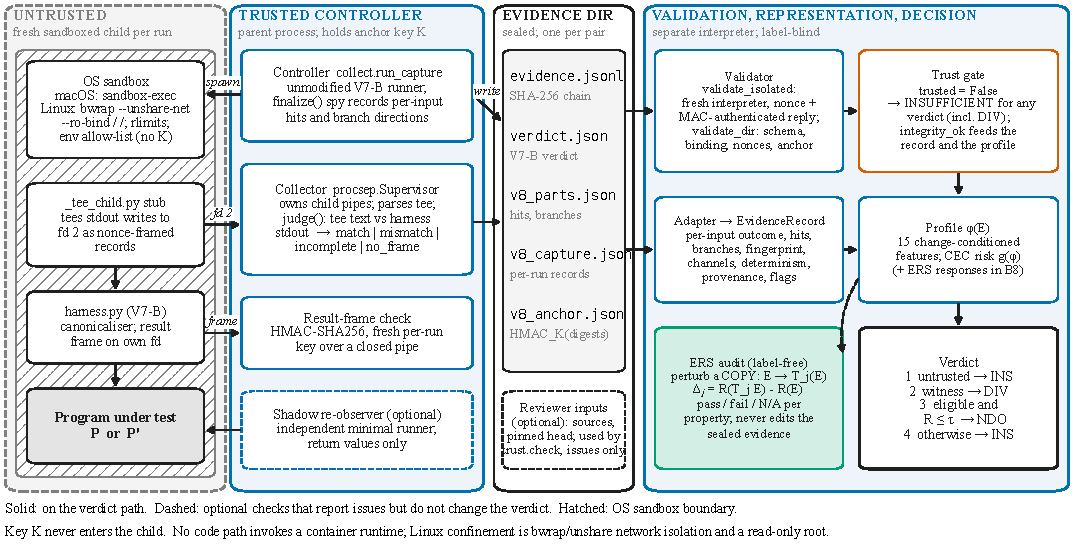
\includegraphics[width=\textwidth]{figures/fig_architecture.pdf}
\caption{\sbg{} architecture as implemented. Each run of $P$ or $P'$ is a fresh sandboxed child. The trusted controller holds the anchor key $K$, which never enters the child; captures an independent tee of standard output; and checks the HMAC-authenticated result frame. Validation of the sealed evidence directory gates the verdict. Shadow re-observation and reviewer-supplied inputs feed optional checks that report issues but do not change the verdict.}
\label{fig:architecture}
\end{figure*}

\begin{figure*}[!t]
\centering
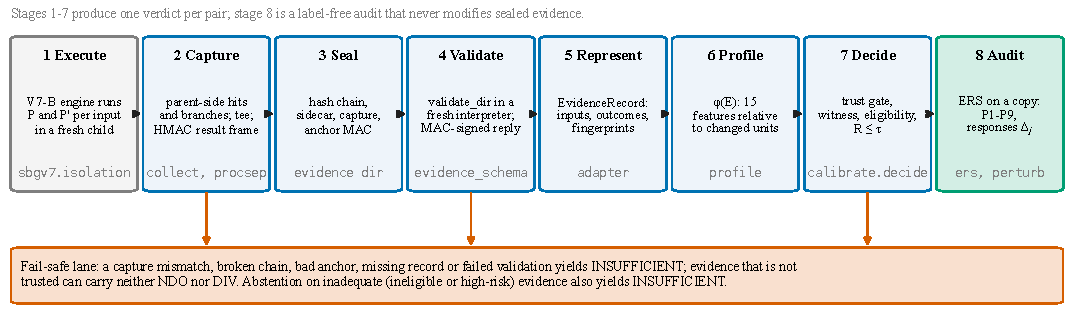
\includegraphics[width=\textwidth]{figures/fig_evidence_lifecycle.pdf}
\caption{Evidence lifecycle for one change pair, with the implementing module under each stage. Any failure in capture, sealing or validation, and any abstention on inadequate evidence, leads to \INS{} (lower lane). Stage~8 is a label-free audit that operates on copies.}
\label{fig:lifecycle}
\end{figure*}

\begin{table*}[!t]
\caption{Component responsibilities. ``Verdict path'' marks components whose output can change the verdict; the remaining components report only.}
\label{tab:components}
\centering
\scriptsize
\setlength{\tabcolsep}{3pt}
\begin{tabular}{|L{2.6cm}|L{3.3cm}|L{6.0cm}|L{2.2cm}|c|}
\hline
Component & Module & Responsibility & Trust role & Verdict path \\
\hline
Evaluated process & V7-B isolation child; \bcode{\_tee\_child.py} & Runs $P$ or $P'$ on one input; the stub tees every standard-output write to fd~2 as a nonce-framed record & Untrusted (A1) & -- \\
OS sandbox & \bcode{sandbox-exec} (macOS); \bcode{bwrap}/\bcode{unshare} (Linux) & Denies network, confines writes; rlimits and environment allow-list exclude $K$ & Containment & -- \\
Controller & \bcode{collect.run\_capture} & Runs the unmodified engine; a spy on the engine's finalisation records per-input hits and branch directions & Trusted & Yes \\
Supervisor & \bcode{procsep.Supervisor} & Spawns children with per-run nonce; parses tee records; \bcode{judge}: match, mismatch, incomplete, no frame & Trusted & Yes \\
Result channel & V7-B result frame & HMAC-SHA256 under a per-run key passed over a pipe closed before user code runs & Authenticated & Yes \\
Evidence directory & \bcode{evidence.jsonl}, \bcode{verdict.json}, \bcode{v8\_parts.json}, \bcode{v8\_capture.json}, \bcode{v8\_anchor.json} & Hash-chained log; hit sidecar bound to the log head; per-run capture record; anchor $\mathrm{HMAC}_K$ over the file digests & Sealed & -- \\
Validator & \bcode{evidence\_schema.validate\_dir}; \bcode{procsep.validate\_isolated} & Schema, binding, contiguity, nonce, per-run status and anchor checks; the isolated variant runs in a fresh interpreter with a MAC-authenticated reply & Trusted & Yes \\
Trust gate & \bcode{procsep.decide}; \bcode{calibrate.Model.decide} & Untrusted evidence yields \INS{} for any engine verdict, including \DIV{} & Trusted & Yes \\
Adapter & \bcode{adapter.load\_record} & Builds the evidence record; sets $\iota$ from engine verification, sidecar consistency and the validator & Trusted & Yes \\
Profile & \bcode{profile.build\_profile} & Computes the 15 change-conditioned features (Table~\ref{tab:profile}) & Label-free & Yes \\
Eligibility & \bcode{policy}; \bcode{calibrate.is\_eligible} & Applies the blocker policy (v8.0, v8.0s, v8.1) & Label-free & Yes \\
CEC & \bcode{calibrate.fit\_select}, \bcode{Model} & Sign-constrained logistic risk model; penalty by inner grouped CV & Uses labels at fit time & Yes \\
Threshold & \bcode{stats.select\_threshold} & Largest prefix whose cluster-bootstrap upper risk bound is $\le\alpha$ & Uses labels at fit time & Yes \\
ERS audit & \bcode{ers.compute\_ers}; \bcode{perturb.apply} & Applies $T_j$ to a copy; records $\Delta_j$, verdicts and pass/fail/N/A & Label-free & No (features in B8) \\
Reviewer checks & \bcode{trust.check} & Shadow re-observation, source binding, pinned log head & Optional & No \\
\hline
\end{tabular}
\end{table*}

\subsection{Evidence Acquisition and Sealing}
Algorithm~\ref{alg:acquire} summarises \code{collect.run\_capture}. Each run of the engine is supervised so that the controller holds an independent record of what every evaluated process wrote. The sidecar records which lines and branch directions every input executed on each side. The capture record lists every spawned run with its nonce, status and output digest.

\begin{algorithm}[!t]
\caption{Evidence acquisition and sealing}
\label{alg:acquire}
\small
\begin{algorithmic}[1]
\Statex \textit{Implements:} \bcode{collect.run\_capture}
\Require base $P$, variant $P'$, entry point, inputs $I$, limits, directory $d$, optional key $K$
\State install a spy on the engine's finalisation step to record per-input outcome, line hits and branch directions
\State open a supervisor session: fresh session nonce; replace the engine's child launcher
\For{each run requested by the engine}
  \State spawn a fresh sandboxed child with the tee stub and a per-run nonce; key $K$ is not in its environment
  \State the stub tees standard output to fd~2 as nonce-framed records; the harness returns an HMAC-authenticated result frame
  \State \Call{judge}{tee text, harness-reported output} $\in\{\textit{match},\textit{mismatch},\textit{incomplete},\textit{no\_frame}\}$
\EndFor
\State $\mathit{out}\gets$ unmodified V7-B comparison of $P$ and $P'$ on $I$ \Comment{hash-chained \code{evidence.jsonl}, verdict}
\State write sidecar: hits, branches, static branches, log head, SHA-256 of the log
\State write capture record: session, configuration and stub digests, one entry per run, trusted flag and reasons
\If{$K$ is configured} write anchor $\mathrm{HMAC}_K(\text{digests of all evidence files})$ \EndIf
\State $\mathit{val}\gets$ \Call{ValidateDir}{$d,K$} \Comment{Algorithm~\ref{alg:validate}}
\If{$\mathit{val}.\mathit{trusted}=\textsf{false}$} \Return verdict \INS{} with the engine verdict and reasons recorded
\Else{} \Return $\mathit{out}$
\EndIf
\end{algorithmic}
\end{algorithm}

\begin{algorithm}[!t]
\caption{Integrity validation}
\label{alg:validate}
\small
\begin{algorithmic}[1]
\Statex \textit{Implements:} \bcode{evidence\_schema.validate\_dir}
\Function{ValidateDir}{$d$, $K$, \textit{requireAnchor}}
\State $\mathit{reasons}\gets\emptyset$
\State check the sidecar schema and its binding to the log head and log digest
\State check the capture record: schema, session, sequence contiguity, per-run nonce uniqueness, per-run status, timings and output digests
\If{$K$ given} verify the anchor MAC over all file digests; a missing or altered anchor adds a reason
\ElsIf{\textit{requireAnchor}} add reason ``anchor required''
\EndIf
\If{$\mathit{reasons}\neq\emptyset$} \Return \textit{trusted} $=\textsf{false}$
\ElsIf{no capture record exists} \Return \textit{trusted} $=\textsf{none}$ \Comment{legacy evidence; not counted as untrusted}
\Else{} \Return \textit{trusted} $=\textsf{true}$
\EndIf
\EndFunction
\State \textit{Record level} (\code{adapter.load\_record}): $\iota(\Ev)=1$ iff the engine's hash chain verifies, the sidecar is consistent and \textit{trusted} $\neq\textsf{false}$
\State \textit{Isolated variant} (\code{procsep.validate\_isolated}): run \Call{ValidateDir}{} in a fresh interpreter; the request carries a fresh nonce and channel key; any timeout, crash, malformed reply, MAC or nonce mismatch yields \textit{trusted} $=\textsf{false}$.
\end{algorithmic}
\end{algorithm}

\subsection{Change-Conditioned Evidence Profile}
The profile is \emph{change-conditioned}: every quantity is computed relative to the changed units $U_c$ rather than to the program as a whole. Let $C\subseteq I$ be the \emph{clean} inputs: non-duplicate inputs whose outcome is \code{SAME}, that are deterministic and that are not lossy. For an input $i$, let $h(i)$ be the changed units it executed. Table~\ref{tab:profile} lists the fifteen features. Three are central.

\emph{Activation} is the share of changed units executed by clean inputs:
\begin{equation}
a(\Ev)=\frac{\left|\bigcup_{i\in C}h(i)\right|}{|U_c|}.
\label{eq:act}
\end{equation}
\emph{Multiplicity} is the number of observationally distinct clean inputs that reached each changed unit:
\begin{equation}
\mu_u=\left|\{\mathit{fp}(i):i\in C,\ u\in h(i)\}\right|,\qquad\mu_{\min}=\min_{u\in U_c}\mu_u.
\label{eq:mu}
\end{equation}
Multiplicity separates ``the change was reached'' from ``the change was reached in several observably different ways''. Counting fingerprints rather than inputs makes it insensitive to repeated identical observations; an input without a fingerprint is never treated as equal to another.

\emph{Effective diversity} $n_{\mathit{eff}}$ is the number of distinct fingerprints among clean inputs. Its provenance-qualified variant counts distinct (fingerprint, provenance) pairs among inputs whose provenance is trusted and not label-derived.

\begin{table}[!t]
\caption{Evidence profile $\prof(\Ev)$ as implemented (\code{sbgv8/profile.py}). Count features enter the model as $\log(1+x)$. ``Const.'' marks features that were constant on the development corpus.}
\label{tab:profile}
\centering
\scriptsize
\setlength{\tabcolsep}{3pt}
\begin{tabular}{|L{2.3cm}|L{3.4cm}|L{1.5cm}|}
\hline
Feature & Definition & Dimension \\
\hline
\code{act\_frac} & Share of $U_c$ executed by clean inputs, Eq.~\eqref{eq:act} & Activation \\
\code{branch\_cov\_min} & Min.\ over sides of observed branch directions on changed lines, relative to $2\times$ static branches & Coverage \\
\code{mu\_min}, \code{mu\_mean} & Min.\ and mean of $\mu_u$, Eq.~\eqref{eq:mu} & Multiplicity \\
\code{n\_same} & $|C|$ & Quantity \\
\code{n\_rep} & Repeat, replay and alternative runs over $C$ & Repetition \\
\code{obs\_react} & Share of $U_c$ reached by a clean, non-degenerate input with a captured channel (a reachability proxy, not a dependence analysis) & Influence \\
\code{n\_eff} & Distinct fingerprints in $C$ & Diversity \\
\code{n\_eff\_prov} & Distinct (fingerprint, provenance) pairs with trusted provenance & Diversity \\
\code{repro\_frac} & Share of deterministic inputs & Reproducibility \\
\code{lossy\_frac} & Share of lossy or degenerate inputs & Loss \\
\code{chan\_complete} & Mean share of declared channels captured & Channels \\
\code{prov\_ok} & All inputs trusted, non-label-derived (const.) & Provenance \\
\code{integrity\_ok} & $\iota(\Ev)$ (const.) & Integrity \\
\code{env\_ok} & $\varepsilon(\Ev)$ (const.) & Environment \\
\hline
\end{tabular}
\end{table}

Two limitations of the profile matter for interpreting the results. First, \code{obs\_react} records that a changed unit was reached by an input whose output was captured, not that the unit's effect propagated to that output; dynamic dependence or checked coverage~\cite{schuler2011assessing} would be the principled replacement. Second, the current adapter does not populate provenance and environment from the runs: they default to ``trusted'' and ``consistent'', and every development record passed integrity validation. These three features were constant on the development corpus, and their effect is examined only through perturbations P7--P9.

\paragraph*{A profile defect found by \ers{}} In the evaluated version, quantity and diversity features counted all non-duplicate inputs, including inputs that reached no changed unit. Irrelevant inputs could therefore raise $n_{\mathit{same}}$, $n_{\mathit{rep}}$ and $n_{\mathit{eff}}$. Perturbation P2 exposed this defect (Section~\ref{sec:results}). The fix restricts every feature to \emph{relevant} evidence, meaning inputs that reach at least one changed unit, and collapses unflagged copies into one evidence class. Statistical results are reported for the pre-fix profile, with the effect of the fix stated alongside.

\subsection{Change-Conditioned Evidence Calibration}
Fig.~\ref{fig:cec} and Algorithm~\ref{alg:cec} describe \cec{}. The risk model $g$ is an $L_2$-penalised logistic regression of the label on the standardised profile, fitted on eligible labelled pairs only. Sign constraints declared before fitting encode domain knowledge: every evidence feature may only lower the estimated risk, and the loss share may only raise it. The constraints are enforced as box bounds in L-BFGS-B. In the full model (B8), the \ers{} responses $\Delta_j$ enter as additional features with free sign; they are computed for each fold from that fold's model without \ers{} features.

The threshold rule makes no exchangeability assumption at the pair level, but it gives no finite-sample guarantee either. A conformal risk-control variant~\cite{angelopoulos2024conformal} is implemented as an exploratory option only, because project-clustered data violate the exchangeability it requires.

\begin{figure*}[!t]
\centering
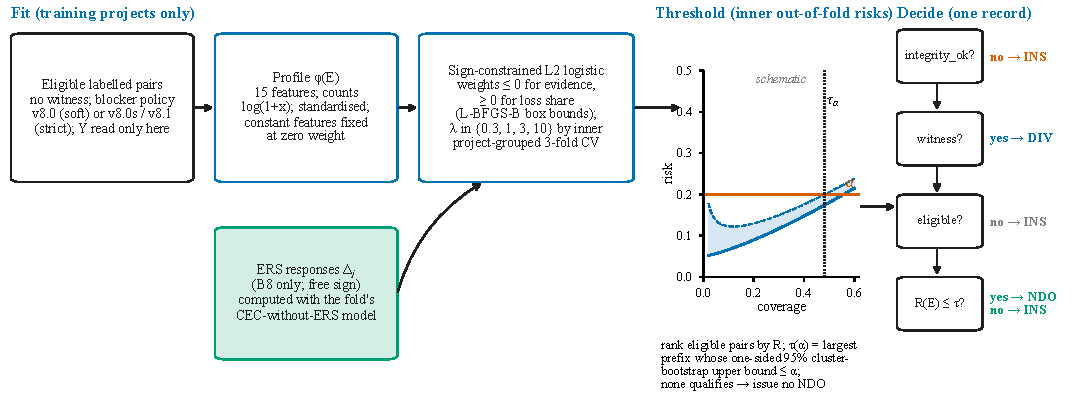
\includegraphics[width=\textwidth]{figures/fig_cec_method.pdf}
\caption{Change-conditioned evidence calibration. Fit: labels are read only for eligible training pairs. Threshold: chosen on inner out-of-fold risks with a one-sided project-cluster bootstrap bound (the inset is schematic, not data). Decide: the per-record procedure of Eq.~\eqref{eq:V}.}
\label{fig:cec}
\end{figure*}

\begin{algorithm}[!t]
\caption{CEC fit and threshold}
\label{alg:cec}
\small
\begin{algorithmic}[1]
\Statex \textit{Implements:} \bcode{calibrate.fit\_select}, \bcode{stats.select\_threshold}
\Require eligible labelled training records $\{(\Ev_k,Y_k,\mathit{proj}_k)\}$, features $\mathcal{F}$, target $\alpha$, resamples $B$
\State $x_k\gets$ standardise($\prof(\Ev_k)$), with $\log(1+\cdot)$ on count features; features constant in training are fixed at weight 0
\For{$\lambda\in\{0.3,1,3,10\}$}
  \State inner project-grouped 3-fold CV: fit sign-constrained logistic loss $+\lambda\|w\|^2$ (L-BFGS-B box bounds); record out-of-fold log loss
\EndFor
\State $\lambda^\ast\gets$ minimiser of out-of-fold log loss; refit $g$ on all training records
\State $s_k\gets$ inner out-of-fold risks; sort eligible records by $s_k$ ascending; group tied scores
\For{$b=1,\dots,B$} draw project clusters with replacement; compute the risk of every prefix under the resample weights \EndFor
\State $\mathit{ub}(t)\gets$ 95th percentile over $b$ of the prefix risk ending at tie-group $t$
\If{$\{t:\mathit{ub}(t)\le\alpha\}=\emptyset$} $\tau_\alpha\gets-\infty$ \Comment{no \NDO{} will be issued}
\Else{} $\tau_\alpha\gets$ score of the largest such prefix
\EndIf
\State \Return $(g,\tau_\alpha)$
\end{algorithmic}
\end{algorithm}

\begin{algorithm}[!t]
\caption{Verdict generation}
\label{alg:decide}
\small
\begin{algorithmic}[1]
\Statex \textit{Implements:} \bcode{calibrate.Model.decide}
\Require evidence record $\Ev$, model $g$, threshold $\tau_\alpha$, blocker policy
\State $r\gets g(\prof(\Ev))$
\If{$\iota(\Ev)=0$} \Return (\INS{}, 1.0) \Comment{trust gate: untrusted evidence carries no conclusion}
\EndIf
\If{a confirmed, reproducible witness exists} \Return (\DIV{}, $r$) \EndIf
\If{$\textsf{elig}(\Ev)$ \textbf{and} $r\le\tau_\alpha$} \Return (\NDO{}, $r$) \EndIf
\State \Return (\INS{}, $r$)
\end{algorithmic}
\end{algorithm}

The order of the first two tests is deliberate. The predecessor checks for a witness first, so a witnessed divergence survives evidence that failed validation. \sbg{} checks integrity first: an \ers{} run showed that a witness on tampered evidence is still a conclusion drawn from untrusted data (Section~\ref{sec:results}). The cost is that tampering can deny a true divergence; it can never manufacture an assurance.

\subsection{Cost and Complexity}\label{sec:cost}
Table~\ref{tab:cost} gives the asymptotic cost of each stage, read from the implementation, with $n$ inputs per record, $u$ changed units, $h$ lines hit per input, $N$ records, $d$ profile features, $J$ perturbations, $B$ bootstrap resamples and $L$ bytes of evidence. Only collection executes programs. Everything downstream of the sealed record is cheap: in this study $n\le12$, $u$ has median 2, $d\le15$ and $N=312$. The statistical stages are dominated by the $B\times N$ resampling weight matrix, about 21\,MB at $B=10{,}000$.

The only measured cost is collection wall time, which the run records store per pair. It had median 2.8\,s, 90th percentile 3.6\,s and maximum 20.3\,s per pair, 932\,s in total for 312 pairs. These runs were not a performance experiment: they ran on a shared host whose one-minute load average was 5.9--9.0, and they included the predecessor's determinism and replay repeats. We therefore report them as indicative only and make no overhead claim against a baseline harness.

\begin{table}[!t]
\caption{Cost of each stage (from the code; no new measurement). Times in the last row are descriptive statistics of existing run records.}
\label{tab:cost}
\centering
\scriptsize
\setlength{\tabcolsep}{2.5pt}
\begin{tabular}{|L{2.1cm}|L{2.4cm}|L{3.2cm}|}
\hline
Stage & Time & Note \\
\hline
Collection (Alg.~\ref{alg:acquire}) & $O(n\cdot r)$ program runs per side & $r$ = configured determinism, replay and alternate-input repeats; dominates total cost \\
Validation (Alg.~\ref{alg:validate}) & $O(L)$ & Hashing and schema checks; isolated mode adds one interpreter start \\
Profile & $O(u\,n\,h)$ & Set intersections of hits with changed units \\
\cec{} fit (Alg.~\ref{alg:cec}) & $O(|\Lambda|\,k\,t\,N d)+O(BN)$ & $|\Lambda|{=}4$, $k{=}3$ inner folds, $t$ L-BFGS-B iterations; threshold bound uses $B{=}1{,}000$ \\
Decision (Alg.~\ref{alg:decide}) & $O(d)$ after the profile & Constant per verdict \\
\ers{} matrix (Alg.~\ref{alg:ers}) & $O(NJ(u\,n\,h+d))$ per predictor & $312\times10\times6=18{,}720$ trials here \\
Matched risk (Alg.~\ref{alg:matched}) & $O(N\log N + BN)$ & $B{=}10{,}000$ for intervals \\
\hline
Observed collection time & \multicolumn{2}{L{5.6cm}|}{Median 2.8\,s, p90 3.6\,s, max 20.3\,s per pair; 932\,s for 312 pairs; host load 5.9--9.0 (\bcode{dev\_records.jsonl}, \code{run\_meta.wall\_s})} \\
\hline
\end{tabular}
\end{table}
